% Created 2022-10-13 Thu 23:26
% Intended LaTeX compiler: pdflatex
\documentclass[11pt]{article}
\usepackage[utf8]{inputenc}
\usepackage[T1]{fontenc}
\usepackage{graphicx}
\usepackage{longtable}
\usepackage{wrapfig}
\usepackage{rotating}
\usepackage[normalem]{ulem}
\usepackage{amsmath}
\usepackage{amssymb}
\usepackage{capt-of}
\usepackage{hyperref}
\author{Alberto Valdez}
\date{\today}
\title{Readme\\\medskip
\large Statistical Analysis with R}
\hypersetup{
 pdfauthor={Alberto Valdez},
 pdftitle={Readme},
 pdfkeywords={},
 pdfsubject={},
 pdfcreator={Emacs 28.1 (Org mode 9.6)}, 
 pdflang={English}}
\begin{document}

\maketitle
\tableofcontents


\section{Statistical Analysis with R}
\label{sec:org46c7723}

In this analysis we will perform multiple tests for finding flaws in the production line of the MechaCar for the CarsRUs company. Then we will propose more tests for the future.

\subsection{Linear Regression to Predict MPG}
\label{sec:org87e7c72}

The first linear regression gives us the following results.

\begin{center}
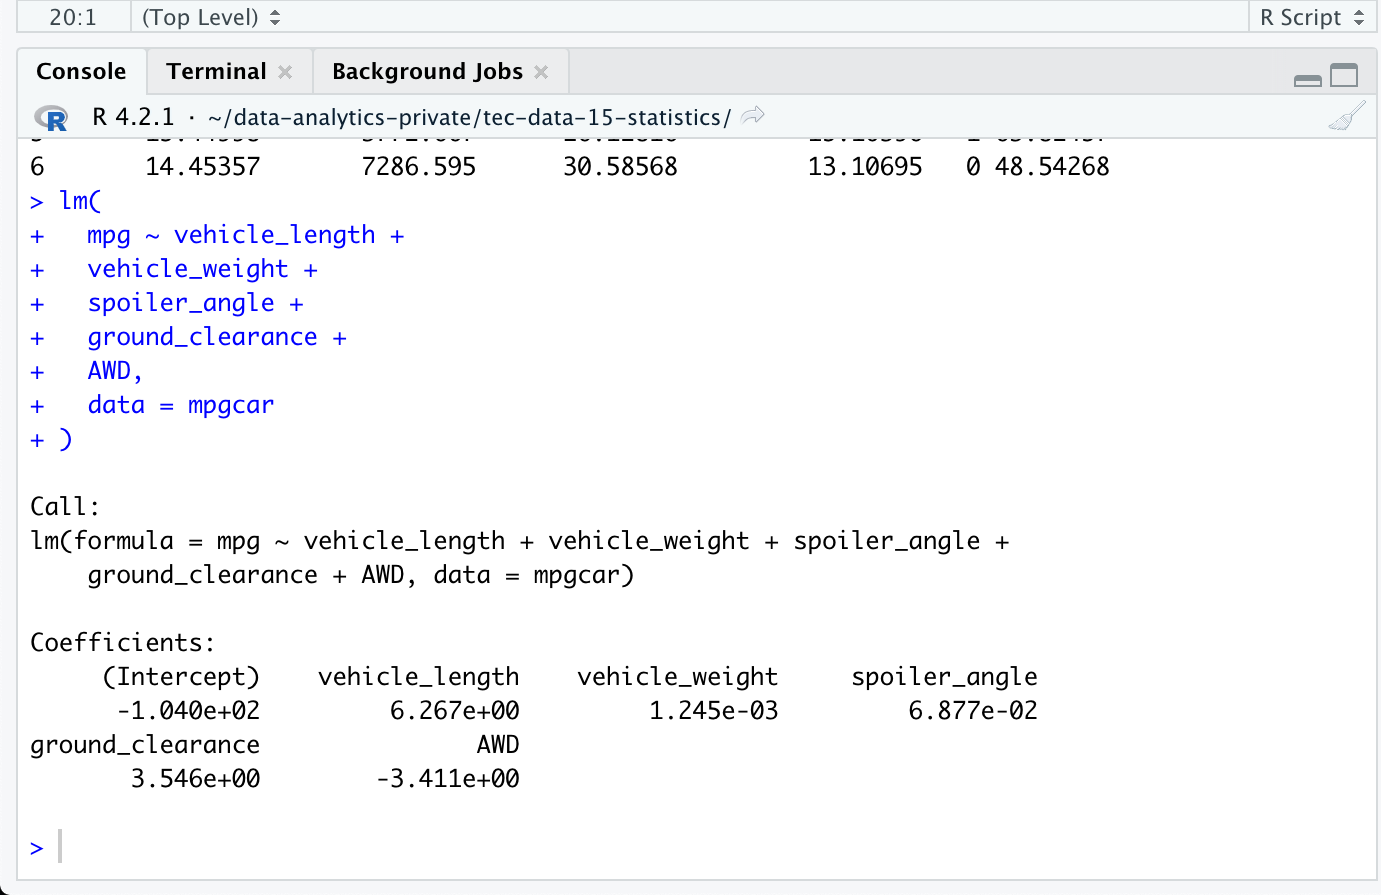
\includegraphics[width=.9\linewidth]{./resources/_r_1.png}
\end{center}

When we call the summary we get our \textbf{p-value} and \textbf{multiple r-square}.

\begin{center}
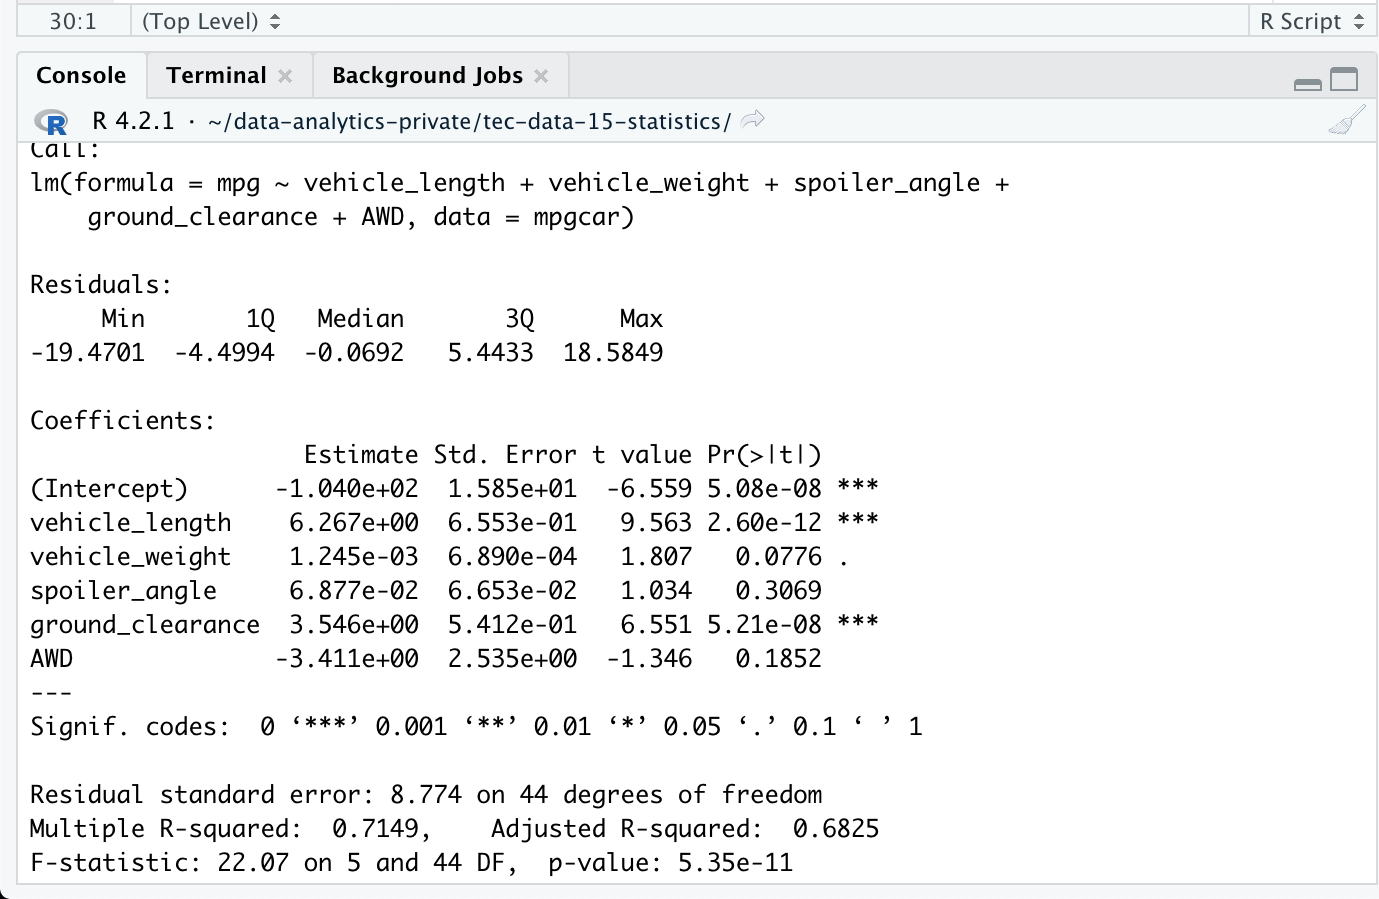
\includegraphics[width=.9\linewidth]{./resources/_r_1b.png}
\end{center}

\begin{enumerate}
\item The coefficients that provide a non-random amount of variance are: vehicle\_length and ground\_clearance (as well as the Intercept) because their \textbf{Pr(>|t|)} value is very small.
\item The slope is not considered zero because the \textbf{r-squared} value is 0.7149, which means the relationship is linear. If we were to plot a line, it would be almost completely perpendicular to both axis.
\item This model is effective on showing us which variables have the most impact (greater correlation) on the \textbf{Milles per Gallon} and which do not affect it as much, so now we can make decisions based on those predictions.
\end{enumerate}


\subsection{Summary Statistics on Suspension Coils}
\label{sec:org4a82521}

These are both summaries on the suspension coils.

\begin{center}
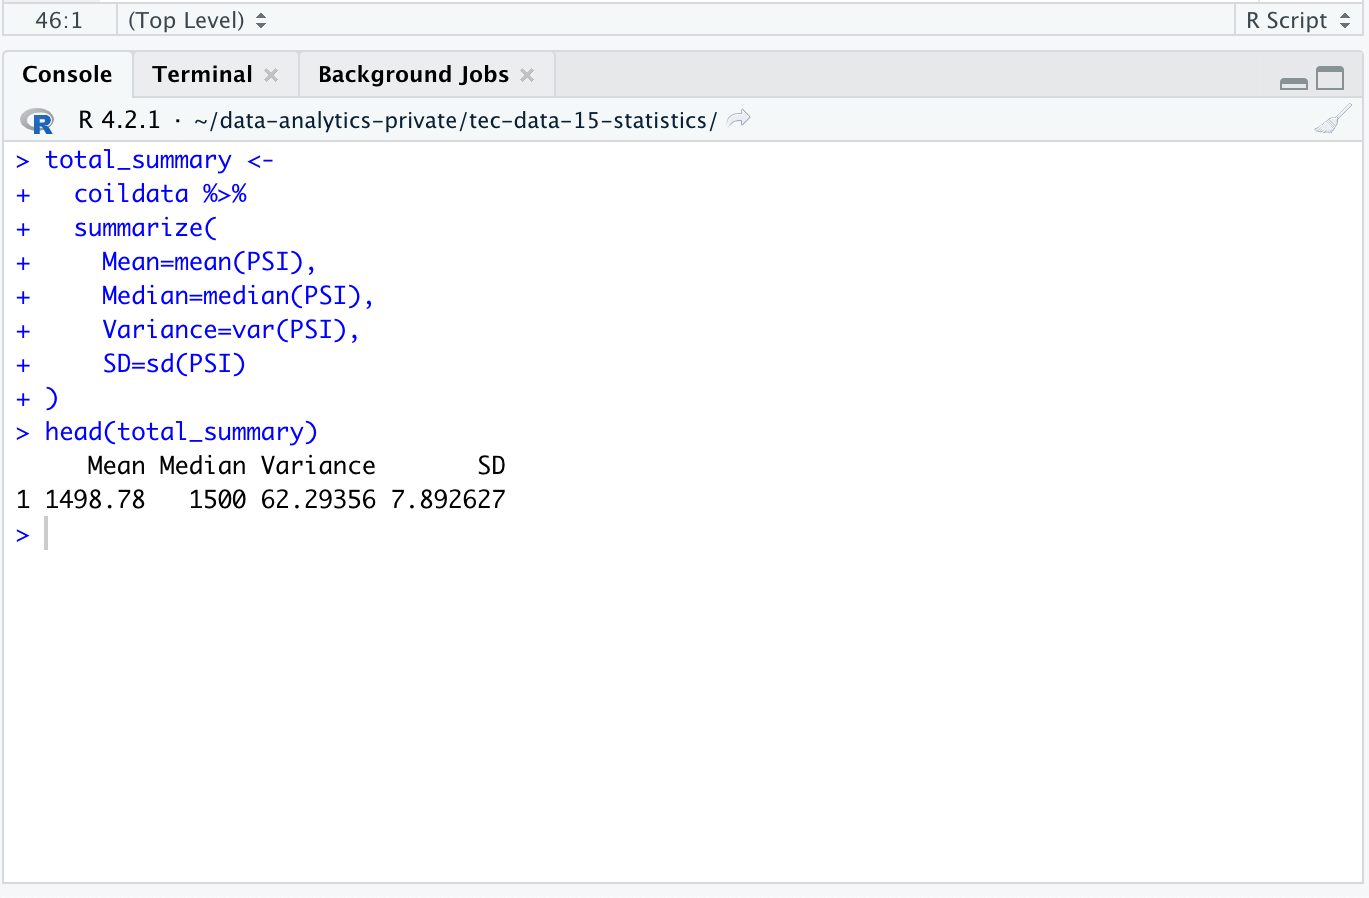
\includegraphics[width=.9\linewidth]{./resources/_r_2.png}
\end{center}

We can see that the total variance on the suspension coils is under 100 pounds per square inch, as per the design specifications. However, when we look at the lots \textbf{individually}, we can see that there is a problem with \texttt{Lot3}.

\begin{center}
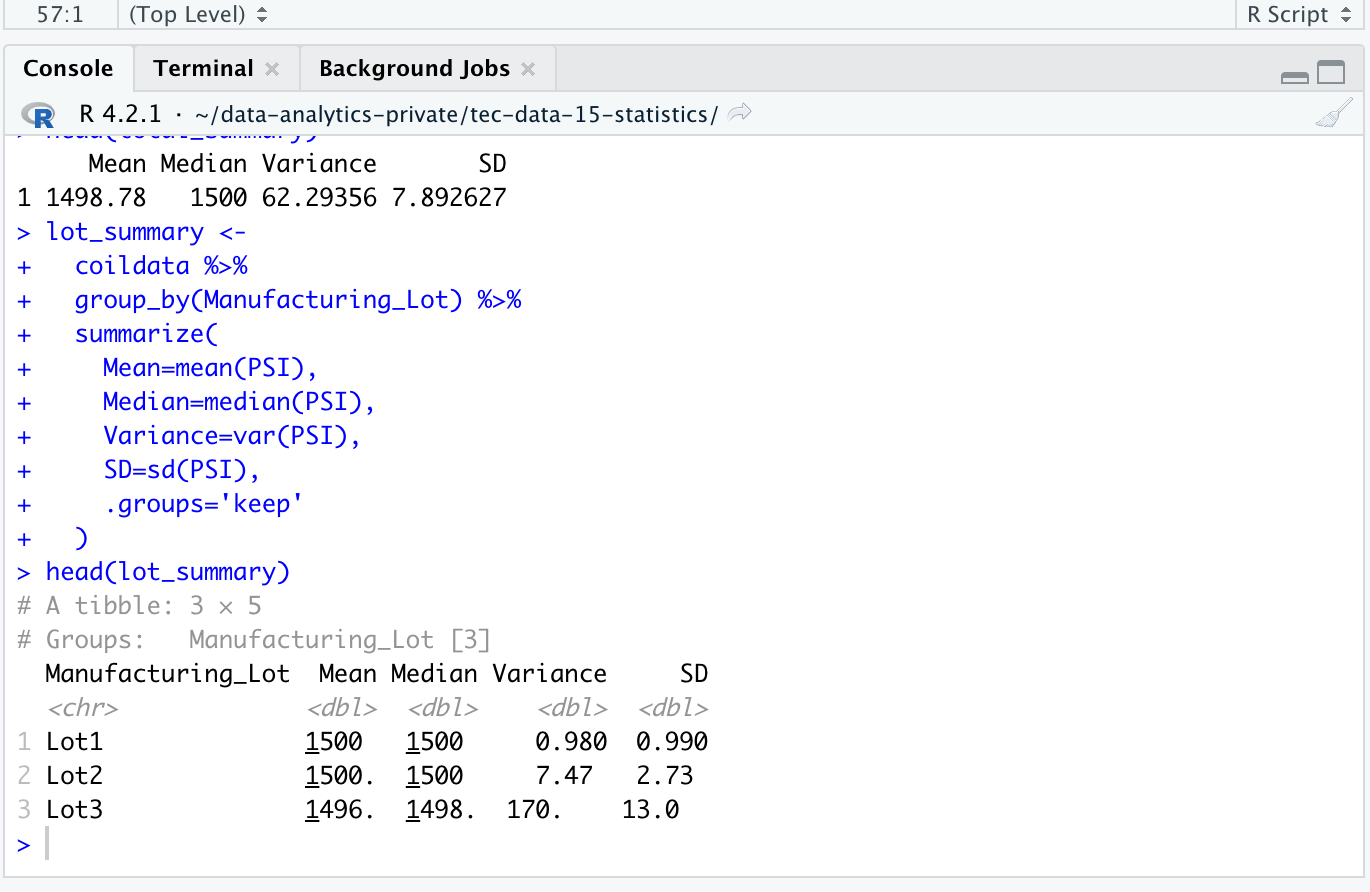
\includegraphics[width=.9\linewidth]{./resources/_r_2b.png}
\end{center}

\texttt{Lot3} doesn't comply with the variance specification, as it's value is \texttt{170}, much higher than the required 100.


\subsection{T-Tests on Suspension Coils}
\label{sec:orgf43d608}

The following tests are made to assert that the mean of each sample is apoximates the population mean. We can verify the measure in our summary table that we have already calculated.

If we compare the mean of the population against itself, we will get a \textbf{p-value} of \texttt{1} because the ratio is perfect.

\begin{center}
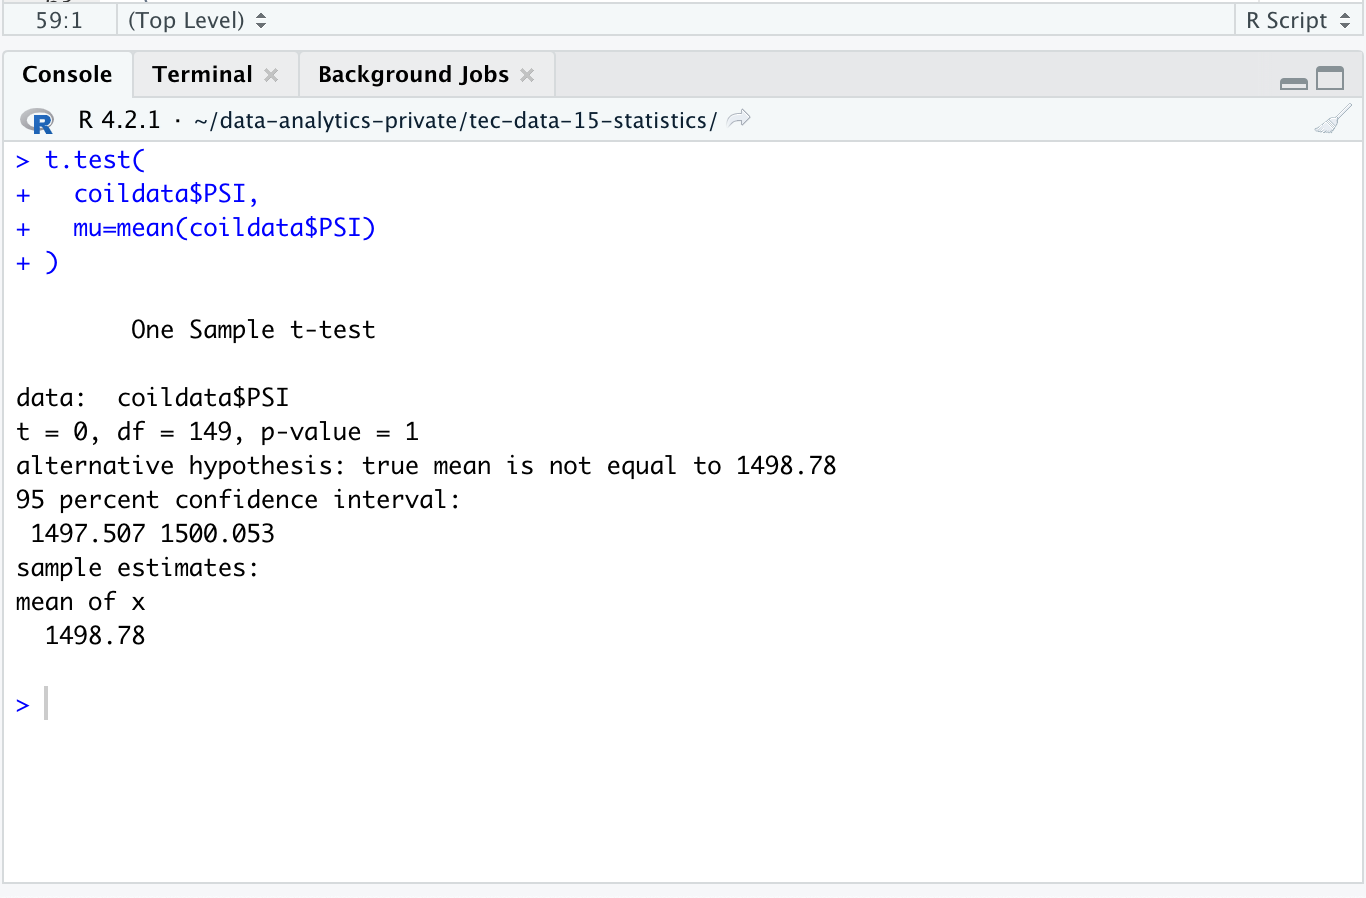
\includegraphics[width=.9\linewidth]{./resources/_r_3a.png}
\end{center}

However, when doing \textbf{one-sample-t-test} for each of the lots, we get a more revealing picture.

Lot1 T-Test

\begin{center}
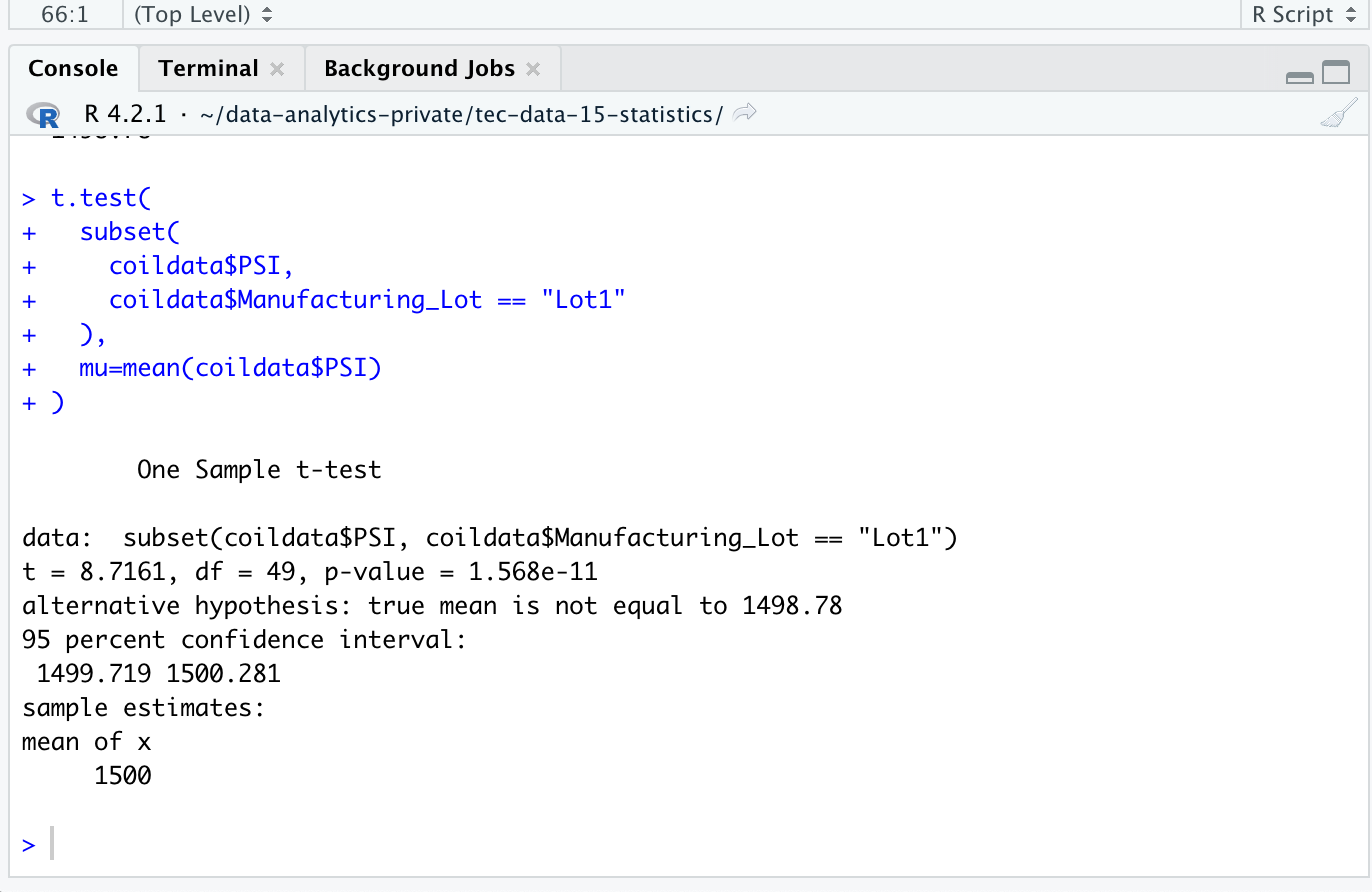
\includegraphics[width=.9\linewidth]{./resources/_r_3b.png}
\end{center}

Lot2 T-Test

\begin{center}
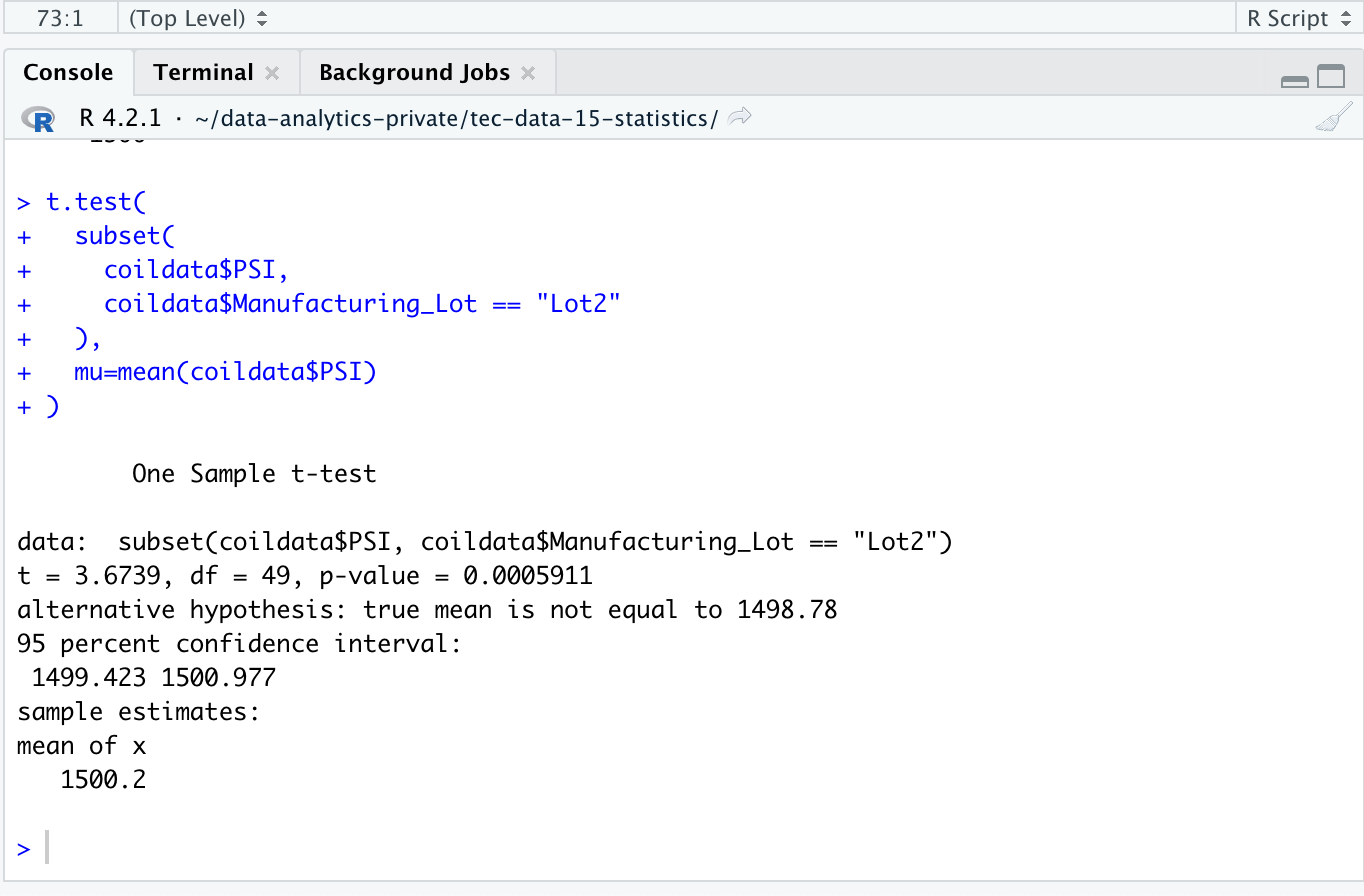
\includegraphics[width=.9\linewidth]{./resources/_r_3c.png}
\end{center}

Lot3 T-Test

\begin{center}
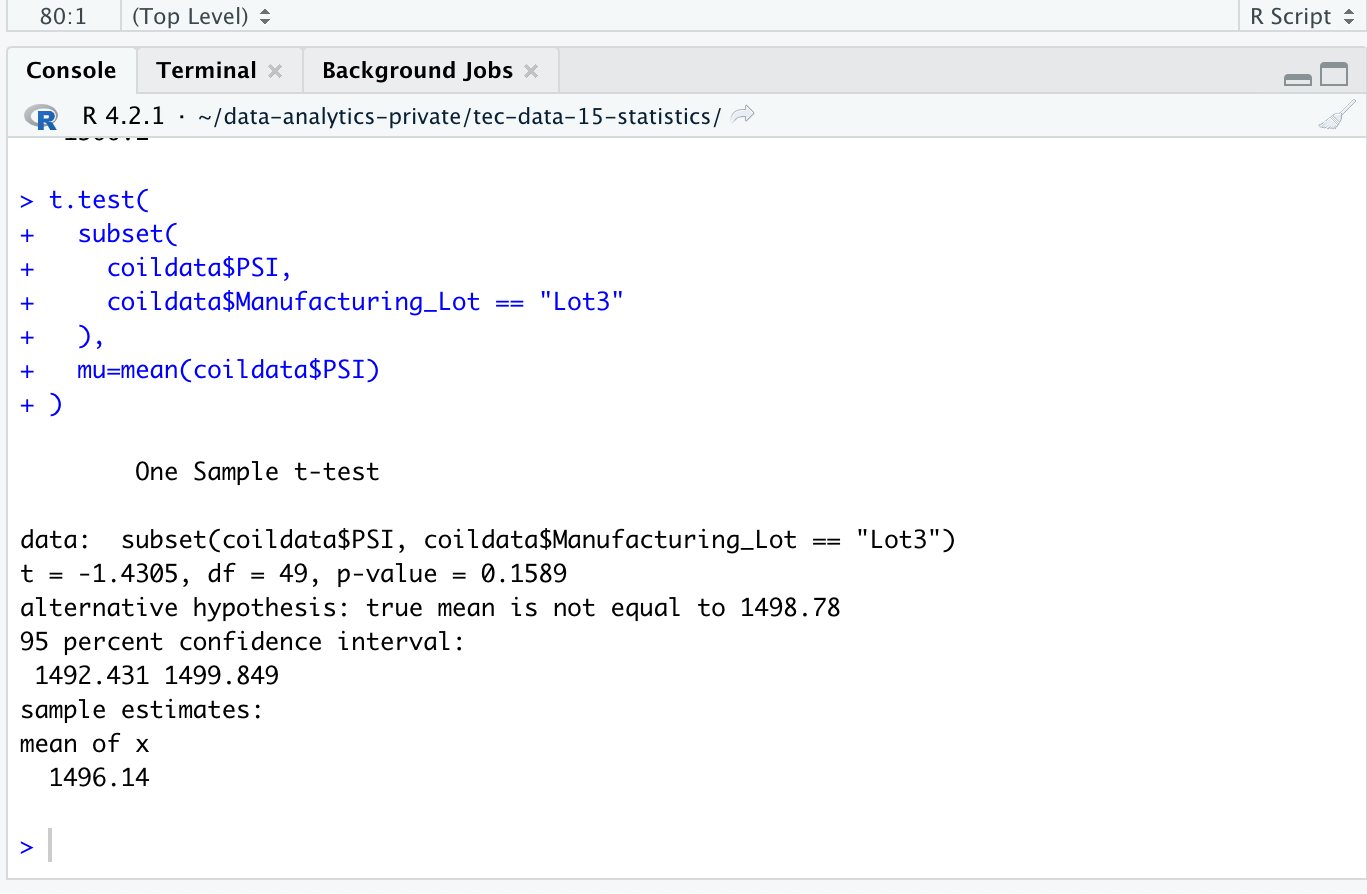
\includegraphics[width=.9\linewidth]{./resources/_r_3d.png}
\end{center}

We can see that the \textbf{p-value} on \texttt{Lot1} and \texttt{Lot2} are within the confidence interval, but the value for \texttt{Lot3} which is equal to \texttt{0.1589} is not, which means this sample deviates from the mean of the population more than we would like it to be.

If our alternative hypothesis is the following:

\begin{quote}
If we measure the mean of the Lot3, it should not deviate from the mean of the population considerably.
\end{quote}

Then we can't validate it, so the null hypothesis would still stand.

\begin{quote}
The mean of the Lot3 will deviate from the population mean considerably when measured.
\end{quote}

\subsection{Study Design: MechaCar vs Competition}
\label{sec:org7ab7dfe}


We want to test the MechaCar product at a larger scale so we should develop a set of tests to help us obtain insight and make predictions about the performance of the product in the market. This means that we have to compare against competitors and include on the consumer as a source for measurements.

We can start with a test to measure safety rating, which would consist of a controlled environment to perform tests on both the MechaCar and its competitors. The null hypothesis will be the following:

\begin{quote}
Given a set of terrains and crash scenarios, the MechaCar won't protect the passengers of the vehicle better than its competitors.
\end{quote}

And the alternative hypothesis will be the following:

\begin{quote}
If we measure damages to test to dummy mannequins and interior of the MechaCar in different crash situations, it will perform better than its competitors in the majority of the tests.
\end{quote}

The measurements we can perform are speed of the vehicles, which will be continuous data, then ordinal data can be severity of the damage in mannequins and interior of the car. We can also measure the PSI on the tires as numerical data.

Given that the number of tests can be scarce, we can do a multiple linear regression on the severity of the interior damage v.s. all the other variables.

For example, given a few numerical variables and a few ordinal variables, we can find a relationship of how much each numerical data affects it. Then we can compare the MechaCar data to other vehicles and look for differences on variance and how consistent each sample is against the population.

\begin{verbatim}
library(tidyverse)
\end{verbatim}

\begin{verbatim}
# mock data
data <- tibble(severity = 1:5, psi = 31:35, speed = 60 + 20*log(severity))
\end{verbatim}

\begin{org}
\begin{center}
\begin{tabular}{rrr}
severity & psi & speed\\
\hline
1 & 31 & 60\\
2 & 32 & 73.8629436111989\\
3 & 33 & 81.9722457733622\\
4 & 34 & 87.7258872223978\\
5 & 35 & 92.188758248682\\
\end{tabular}
\end{center}
\end{org}

The previous data is just a mock to demonstrate how we could perform the tests with R and then use linear regression to find correlation and variance.

\begin{verbatim}
summary(lm(severity ~ psi + speed, data=data))
\end{verbatim}

\begin{verbatim}

Call:
lm(formula = severity ~ psi + speed, data = data)

Residuals:
         1          2          3          4          5
-2.408e-16  8.565e-16 -6.017e-16 -4.030e-16  3.890e-16

Coefficients:
              Estimate Std. Error    t value Pr(>|t|)
(Intercept) -3.000e+01  2.777e-14 -1.080e+15   <2e-16 ***
psi          1.000e+00  1.180e-15  8.473e+14   <2e-16 ***
speed        5.456e-16  1.468e-16  3.716e+00   0.0654 .
---
Signif. codes:  0 ‘***’ 0.001 ‘**’ 0.01 ‘*’ 0.05 ‘.’ 0.1 ‘ ’ 1

Residual standard error: 8.566e-16 on 2 degrees of freedom
Multiple R-squared:      1,	Adjusted R-squared:      1
F-statistic: 6.815e+30 on 2 and 2 DF,  p-value: < 2.2e-16

Warning message:
In summary.lm(lm(severity ~ psi + speed, data = data)) :
  essentially perfect fit: summary may be unreliable
\end{verbatim}

The test will gain relevance if we measure more variables of the environment and the state of the cars as well as including the competition.

The null hypothesis will be negated if the MechaCar performs better and there is less interior damage than its competitors in a majority of the scenarios.
\end{document}
